% vim:ts=2 sw=2 et spell tw=80:

\section{Construction of the Spherical Harmonics}
\kopfrechts{Construction of the Spherical Harmonics}

We have finally arrived at the main section that gives this chapter its name.
The idea is to discuss spherical harmonics, their mathematical origin, some of
their properties and applications.

To begin, we will give an outline of the contents of the rest of this chapter.
The subsection \ref{kugel:sec:construction:eigenvalue} will be devoted to an
eigenvalue problem involving the Laplace operator, through which we will derive
a set of special eigenfunctions, which are the \emph{spherical harmonics}.  In
the subsections from \ref{kugel:sec:construction:orthogonality} to
\ref{kugel:sec:construction:recurrence}, a few interesting properties related to
orthogonality will be discussed. Some of these will come back to help us
understand in more detail why they are useful in various real-world
applications, which will be presented in the section
\ref{kugel:sec:applications}. 

Finally, section \ref{kugel:sec:expansion} is devoted to one of the most
beautiful applications (in our humble opinion), namely the derivation of a
Fourier-style series expansion on the sphere.  This will allow us to connect all
the dots we have created with the previous sections, concluding that Fourier is
just a specific case of the application of the concept of orthogonality. Our
hope is that after reading this section you will appreciate the beauty and power
of generalization that mathematics offers us.

\subsection{Eigenvalue Problem}
\label{kugel:sec:construction:eigenvalue}

From section \ref{kugel:sec:preliminaries:laplacian}, we know that the spherical
Laplacian in the spherical coordinate system (shown in Figure
\ref{kugel:fig:spherical-coordinates}) is defined as
\begin{equation*}
    \sphlaplacian :=
      \frac{1}{r^2} \frac{\partial}{\partial r} \left(
        r^2 \frac{\partial}{\partial r}
      \right)
      + \frac{1}{r^2} \left[
          \frac{1}{\sin\vartheta} \frac{\partial}{\partial \vartheta} \left(
            \sin\vartheta \frac{\partial}{\partial\vartheta}
          \right)
        + \frac{1}{\sin^2 \vartheta} \frac{\partial^2}{\partial\varphi^2}
      \right].
\end{equation*}
But we will not consider this algebraic monstrosity in its entirety. As
previously hinted, we will only care about the \emph{surface} of the sphere.
This is for many reasons, but mainly to simplify reduce the already broad scope
of this text. Concretely, we will always work on the unit sphere, which just
means that we set $r = 1$ and keep only $\vartheta$ and $\varphi$ as free
variables.  Now, since the variable $r$ became a constant, we can leave out all
derivatives with respect to $r$ and substitute all $r$'s with 1's to obtain a
new operator that deserves its own name.

\begin{definition}[Surface spherical Laplacian]
  \label{kugel:def:surface-laplacian}
  The operator
  \begin{equation*}
      \surflaplacian :=
        \frac{1}{\sin\vartheta} \frac{\partial}{\partial \vartheta} \left(
          \sin\vartheta \frac{\partial}{\partial\vartheta}
        \right)
        + \frac{1}{\sin^2 \vartheta} \frac{\partial^2}{\partial\varphi^2},
  \end{equation*}
  is called the surface spherical Laplacian.
\end{definition}

In the definition, the subscript ``$\partial S$'' was used to emphasize the fact
that we are on the spherical surface, which can be understood as being the
boundary of the sphere. But what does it actually do? To get an intuition, first
of all, notice the fact that $\surflaplacian$ is made of second derivatives,
which means that this a measure of \emph{curvature}; But curvature of what? To
get an even stronger intuition we will go into geometry, were curvature can be
grasped very well visually. Consider figure \ref{kugel:fig:curvature} where the
curvature is shown using colors: positive curvature in red, and negative
curvature in blue. First we have the curvature of a curve in 1D, then the
curvature of a surface (2D), and finally the curvature of a function on the
surface of the unit sphere.

\begin{figure}
  \centering
  \subfigure[Curvature in 1D.]
    {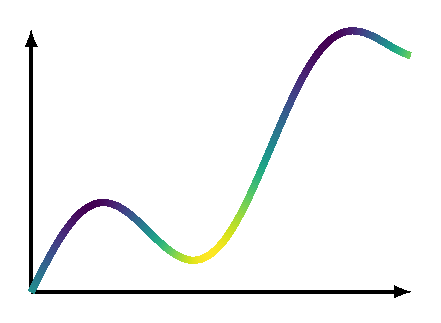
\includegraphics[width=.3\linewidth]{papers/kugel/figures/tikz/curvature-1d}}
  \hskip 5mm
  \subfigure[Curvature on a plane.]
    {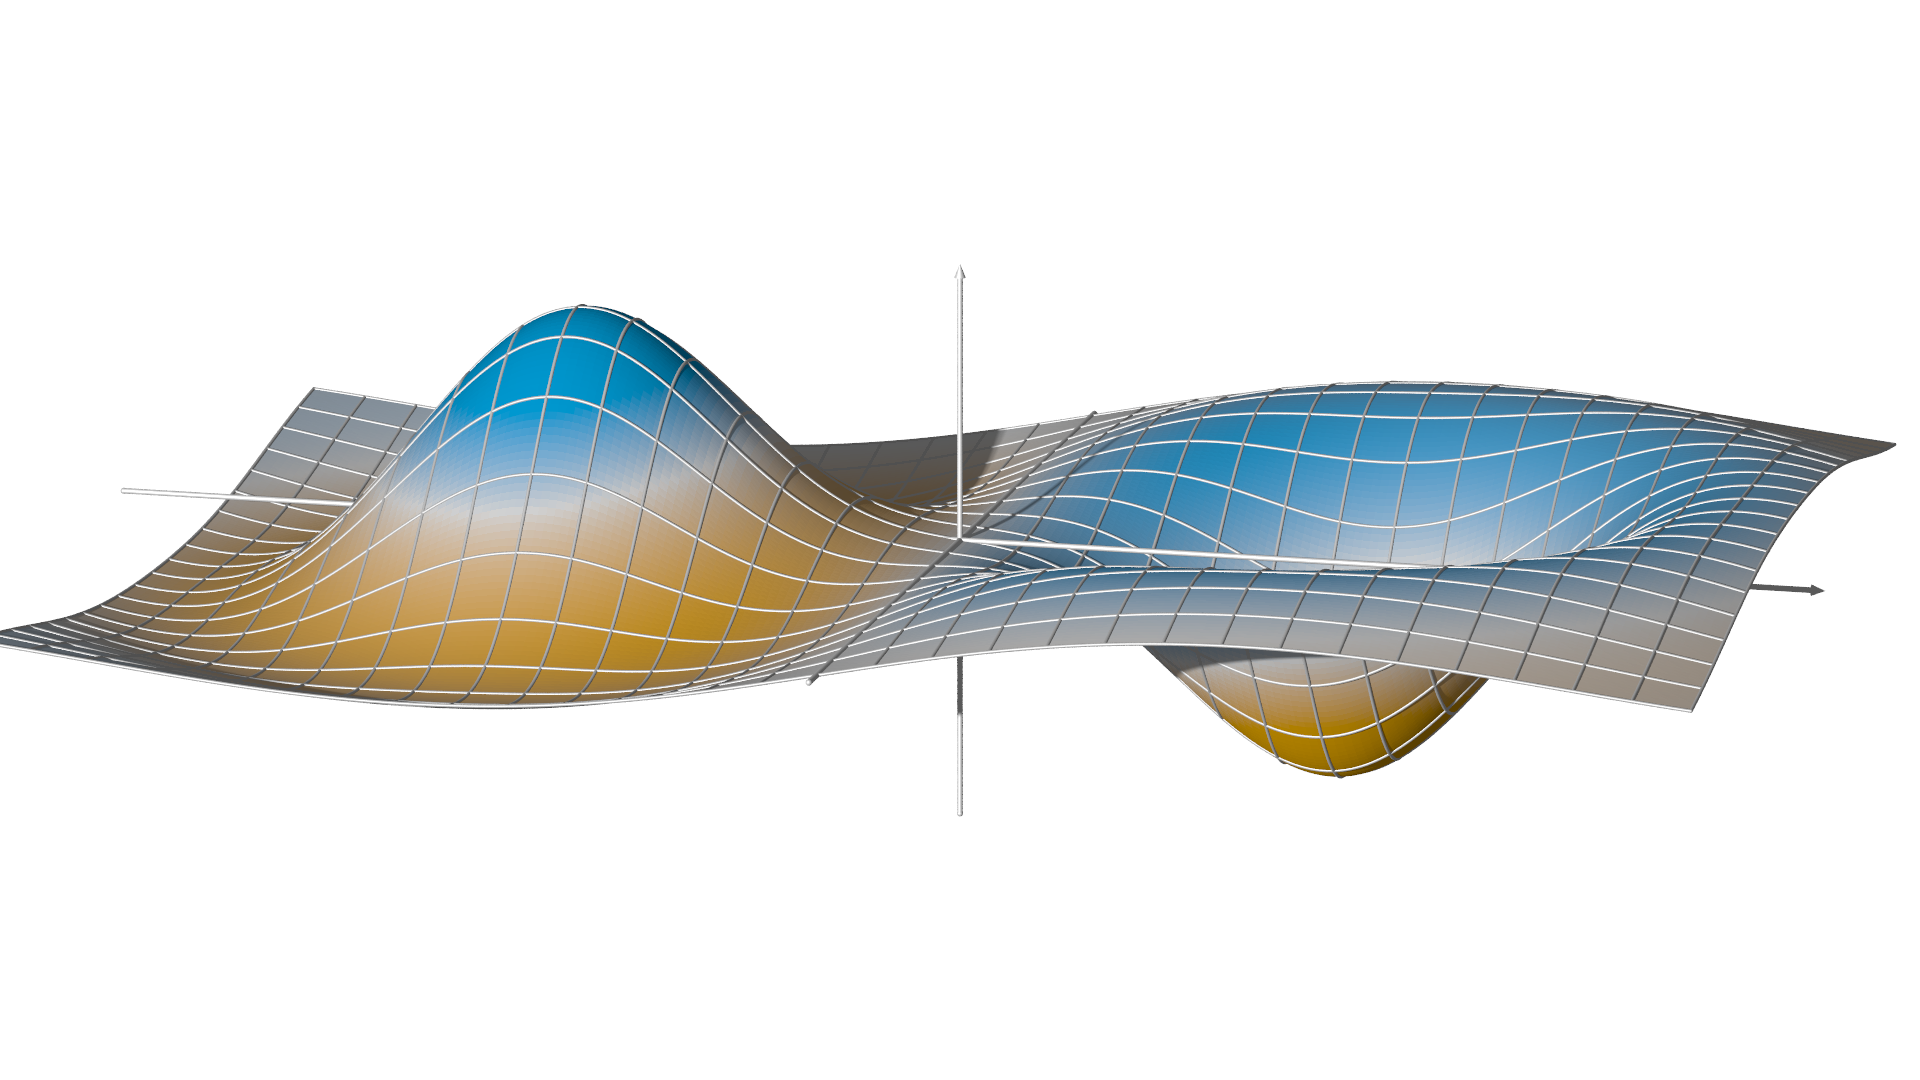
\includegraphics[width=.3\linewidth]{papers/kugel/figures/povray/curvature}}
  \hskip 5mm
  \subfigure[Cuvature on $S^2$.]
    {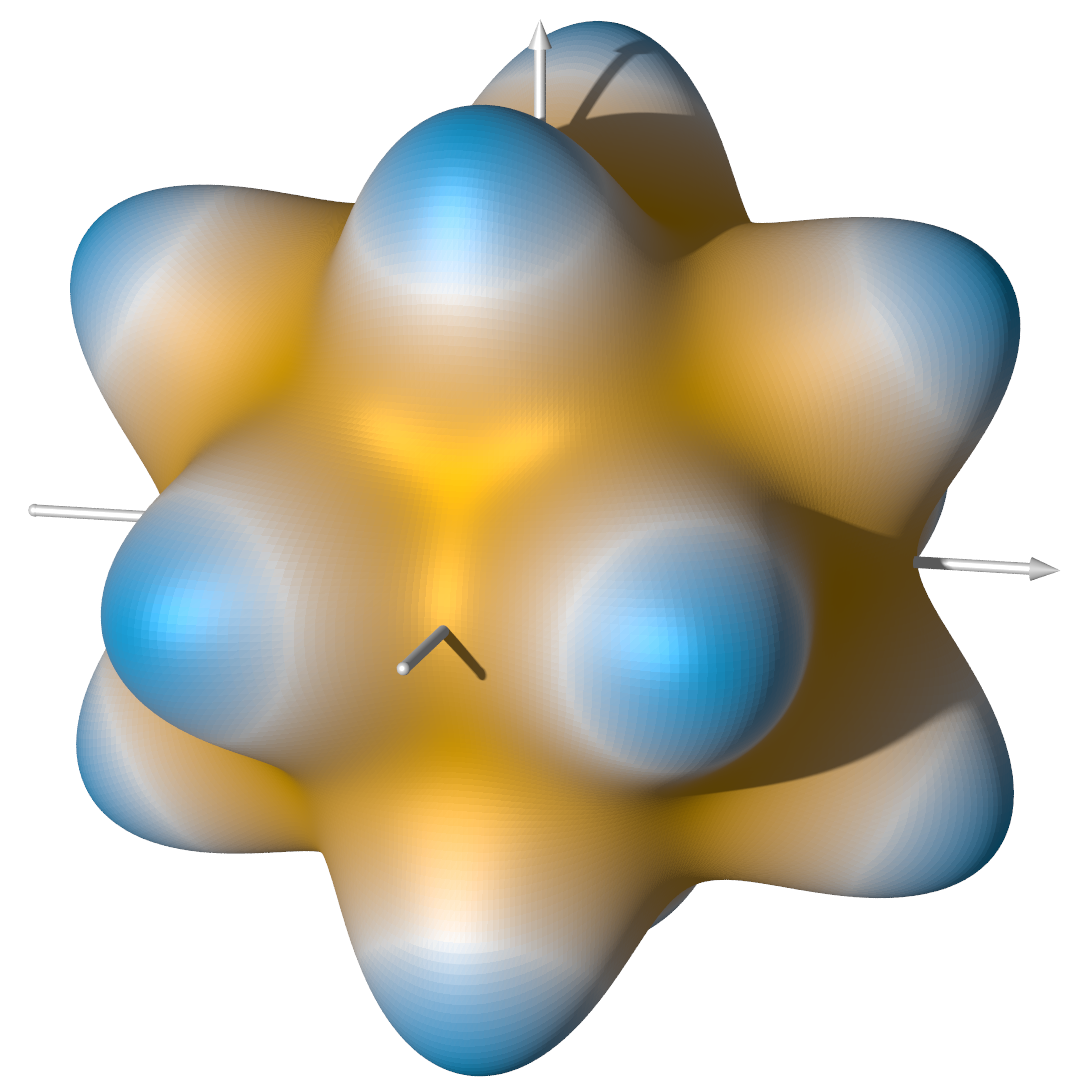
\includegraphics[width=.3\linewidth]{papers/kugel/figures/povray/spherecurve}}
  \caption{
    Curvature.
    \label{kugel:fig:curvature}
  }
\end{figure}

Now that we have defined an operator, we can go and study its eigenfunctions,
which means that we would like to find the functions $f(\vartheta, \varphi)$
that satisfy the equation
\begin{equation} \label{kugel:eqn:eigen}
    \surflaplacian f = -\lambda f.
\end{equation}
Perhaps it may not be obvious at first glance, but we are in fact dealing with a
partial differential equation (PDE)\footnote{Considering the fact that we are
dealing with a PDE, you may be wondering what are the boundary conditions. Well,
since this eigenvalue problem is been developed on the spherical surface
(boundary of a sphere), the boundary in this case are empty, i.e no boundary
condition has to be considered.}. If we unpack the notation of the operator
$\nabla^2_{\partial S}$ according to definition
\ref{kugel:def:surface-laplacian}, we get:
\begin{equation} \label{kugel:eqn:eigen-pde}
    \frac{1}{\sin\vartheta} \frac{\partial}{\partial \vartheta} \left(
      \sin\vartheta \frac{\partial f}{\partial\vartheta}
    \right)
    + \frac{1}{\sin^2 \vartheta} \frac{\partial^2 f}{\partial\varphi^2}
    + \lambda f = 0.
\end{equation}
Since all functions satisfying \eqref{kugel:eqn:eigen-pde} are the
\emph{eigenfunctions} of $\surflaplacian$, our new goal is to solve this PDE.
The task may seem very difficult but we can simplify it with a well-known
technique: \emph{the separation Ansatz}\footnote{See section
\ref{buch:pde:section:separation} for more on separation.}. It consists in
assuming that the function $f(\vartheta, \varphi)$ can be factorized in the
following form:
\begin{equation}
    f(\vartheta, \varphi) = \Theta(\vartheta)\Phi(\varphi). 
\end{equation}
In other words, we are saying that the effect of the two independent variables
can be described using the multiplication of two functions that describe their
effect separately. This separation process was already presented in section
\ref{buch:pde:section:kugel}, but we will briefly rehearse it here for
convenience. If we substitute this assumption in
\eqref{kugel:eqn:eigen-pde}, we have:
\begin{equation*}
    \frac{1}{\sin\vartheta} \frac{\partial}{\partial \vartheta} \left(
      \sin\vartheta \frac{\partial  \Theta(\vartheta)}{\partial\vartheta}
    \right) \Phi(\varphi)
    + \frac{1}{\sin^2 \vartheta}
      \frac{\partial^2 \Phi(\varphi)}{\partial\varphi^2}
      \Theta(\vartheta)
    + \lambda \Theta(\vartheta)\Phi(\varphi) = 0.
\end{equation*}
Dividing by $\Theta(\vartheta)\Phi(\varphi)$ and introducing an auxiliary
variable $m^2$, the separation constant, yields:
\begin{equation*}
  \frac{1}{\Theta(\vartheta)}\sin \vartheta \frac{d}{d \vartheta} \left(
    \sin \vartheta \frac{d \Theta}{d \vartheta}
  \right)
  + \lambda \sin^2 \vartheta
  = -\frac{1}{\Phi(\varphi)} \frac{d^2\Phi(\varphi)}{d\varphi^2}
  = m^2,
\end{equation*}
which is equivalent to the following system of two first order ordinary
differential equations (ODEs):
\begin{subequations}
  \begin{gather}
    \frac{d^2\Phi(\varphi)}{d\varphi^2} = -m^2 \Phi(\varphi),
      \label{kugel:eqn:ode-phi} \\ 
    \sin \vartheta \frac{d}{d \vartheta} \left(
      \sin \vartheta \frac{d \Theta}{d \vartheta}
    \right)
    + \left( \lambda - \frac{m^2}{\sin^2 \vartheta} \right)
      \Theta(\vartheta) = 0
      \label{kugel:eqn:ode-theta}.
  \end{gather}
\end{subequations}
The solution of \eqref{kugel:eqn:ode-phi} is easy to find: The complex
exponential is obviously the function we are looking for. So we can directly
write the solutions
\begin{equation} \label{kugel:eqn:ode-phi-sol}
    \Phi(\varphi) = e^{i m \varphi}, \quad m \in \mathbb{Z}.
\end{equation}
The restriction that the separation constant $m$ needs to be an integer arises
from the fact that we require a $2\pi$-periodicity in $\varphi$ since the
coordinate systems requires that $\Phi(\varphi + 2\pi) = \Phi(\varphi)$.
Unfortunately, solving \eqref{kugel:eqn:ode-theta} is not as straightforward,
actually, it is quite difficult, and the process is so involved that it will
require a dedicated section of its own.

\subsection{Legendre Functions}

\begin{figure}
  \centering
  \subfigure[Spherical coordinates. \label{kugel:fig:spherical-coordinates}]
    {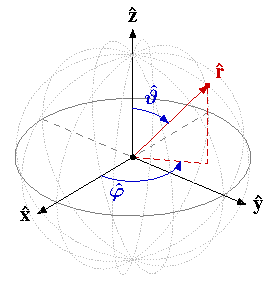
\includegraphics[width=.45\linewidth]{papers/kugel/figures/tikz/spherical-coordinates}}
  \qquad
  \subfigure[Substitution. \label{kugel:fig:legendre-substitution}]
    {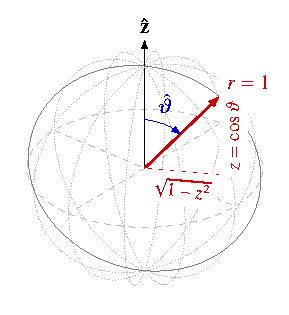
\includegraphics[
      width=.45\linewidth
      % scale = 1.2,
      % trim = 0 40 0 0, clip,
    ]{papers/kugel/figures/tikz/legendre-substitution}}
  \caption{
    (a) Spherical coordinate system. Space is described with the free variables
    $r \in \mathbb{R}_0^+$, $\vartheta \in [0; \pi]$ and $\varphi \in [0;
    2\pi)$. (b) Geometrical intuition for the substitution to obtain the
    Legendre equation.
  }
\end{figure}

To solve \eqref{kugel:eqn:ode-theta} we start with the substitution $z = \cos
\vartheta$, which has a neat geometrical justification. To see it consider
figure \ref{kugel:fig:legendre-substitution}, where we sketched the geometry of
the problem. Algebraically, the operator $\frac{d}{d \vartheta}$ becomes
\begin{equation*}
    \frac{d}{d \vartheta}
    = \frac{dz}{d \vartheta}\frac{d}{dz}
    = -\sin \vartheta \frac{d}{dz}
    = -\sqrt{1-z^2} \frac{d}{dz},
\end{equation*} 
since $\sin \vartheta = \sqrt{1 - \cos^2 \vartheta} = \sqrt{1 - z^2}$, which
agrees with our sketch. Thus, \eqref{kugel:eqn:ode-theta} becomes 
\begin{align*}
  \frac{-\sqrt{1-z^2}}{\sqrt{1-z^2}} \frac{d}{dz} \left[
    \left(\sqrt{1-z^2}\right) \left(-\sqrt{1-z^2}\right) \frac{d \Theta}{dz}
  \right]
  + \left( \lambda - \frac{m^2}{1 - z^2} \right)\Theta(\vartheta) &= 0,
  \\
  \frac{d}{dz} \left[ (1-z^2) \frac{d \Theta}{dz} \right]
  + \left( \lambda - \frac{m^2}{1 - z^2} \right)\Theta(\vartheta) &= 0,
  \\
  (1-z^2)\frac{d^2 \Theta}{dz} - 2z\frac{d \Theta}{dz}
  + \left( \lambda - \frac{m^2}{1 - z^2} \right)\Theta(\vartheta) &= 0.
\end{align*}
By making two final cosmetic substitutions, namely $Z(z) = \Theta(\cos^{-1}z)$
and $\lambda = n(n+1)$, we obtain what is known in the literature as the
\emph{associated Legendre equation} of order $m$:
\nocite{olver_introduction_2013}
\begin{equation} \label{kugel:eqn:associated-legendre}
  (1 - z^2)\frac{d^2 Z}{dz^2}
  - 2z\frac{d Z}{dz}
  + \left( n(n + 1) - \frac{m^2}{1 - z^2} \right) Z(z) = 0,
  \quad
  z \in [-1; 1], m \in \mathbb{Z}.
\end{equation}

Our new goal has therefore become to solve
\eqref{kugel:eqn:associated-legendre}, since if we find a solution for $Z(z)$ we
can perform the substitution backwards and get back to our eigenvalue problem.
However, the associated Legendre equation is not any easier, so to attack the
problem we will look for the solutions in the easier special case when $m = 0$.
This reduces the problem because it removes the double pole, which is always
tricky to deal with\footnote{However, the differential equation is still
singular because of the factor in front of the second derivative.}. In fact, the
reduced problem when $m = 0$ is known as the \emph{Legendre equation}:
\begin{equation} \label{kugel:eqn:legendre}
  (1 - z^2)\frac{d^2 Z}{dz^2}
  - 2z\frac{d Z}{dz}
  + n(n + 1) Z(z) = 0,
  \quad
  z \in [-1; 1].
\end{equation}

The Legendre equation is a second order differential equation, and therefore it
has two independent solutions, which are known as \emph{Legendre functions} of the
first and second kind. For the scope of this text we will only derive a special
case of the former that is known known as the \emph{Legendre polynomials}, since
we only need a solution between $-1$ and $1$.

\begin{lemma}[Legendre polynomials]
  \label{kugel:thm:legendre-poly}
  The polynomial function
  \[
    P_n(z) = \sum^{\lfloor n/2 \rfloor}_{k=0}
      \frac{(-1)^k}{2^n k!} \frac{(2n - 2k)!}{(n - k)! (n-2k)!} z^{n - 2k}
  \]
  is the only finite solution of the Legendre equation
  \eqref{kugel:eqn:legendre} when $n \in \mathbb{Z}$ and $z \in [-1; 1]$.
\end{lemma}
\begin{proof}
  This results is derived in section \ref{kugel:sec:proofs:legendre}.
\end{proof}

Since the Legendre \emph{polynomials} are indeed polynomials, they can also be
expressed using the hypergeometric functions described in section
\ref{buch:rekursion:section:hypergeometrische-funktion}, so in fact
\begin{equation}
  P_n(z) = {}_2F_1 \left( \begin{matrix}
    n + 1, & -n \\ \multicolumn{2}{c}{1}
  \end{matrix} ; \frac{1 - z}{2} \right).
\end{equation}
Further, there are a few more interesting but not very relevant forms to write
$P_n(z)$ such as \emph{Rodrigues' formula} and \emph{Laplace's integral
representation} which are
\begin{equation*}
  P_n(z) = \frac{1}{2^n n!} \frac{d^n}{dz^n} (z^2 - 1)^n,
  \qquad \text{and} \qquad
  P_n(z) = \frac{1}{\pi} \int_0^\pi \left(
    z + \cos\vartheta \sqrt{z^2 - 1}
  \right) \, d\vartheta
\end{equation*}
respectively, both of which we will not prove (see chapter 3 of
\cite{bell_special_2004} for a proof). Now that we have a solution for the
Legendre equation, we can make use of the following lemma to patch the solutions
such that they also become solutions of the associated Legendre equation
\eqref{kugel:eqn:associated-legendre}.

\begin{lemma} \label{kugel:thm:extend-legendre}
  If $Z_n(z)$ is a solution of the Legendre equation \eqref{kugel:eqn:legendre},
  then
  \begin{equation*}
    Z^m_n(z) = (1 - z^2)^{m/2} \frac{d^m}{dz^m}Z_n(z)
  \end{equation*}
  solves the associated Legendre equation \eqref{kugel:eqn:associated-legendre}.
  \nocite{bell_special_2004}
\end{lemma}
\begin{proof}
  See section \ref{kugel:sec:proofs:associated-legendre}.
\end{proof}

What is happening in lemma \ref{kugel:thm:extend-legendre}, is that we are
essentially inserting a square root function in the solution in order to be able
to reach the parts of the domain near the poles at $\pm 1$ of the associated
Legendre equation, which is not possible only using power series (see sections
\ref{buch:differentialgleichungen:section:potenzreihenmethode} and
\ref{buch:differentialgleichungen:subsection:verallgemeinrt} for a discussion).
Now, since we have a solution in our domain, namely $P_n(z)$, we can insert it
in the lemma obtain the \emph{associated Legendre functions}.

\begin{definition}[Ferrers or associated Legendre functions]
  \label{kugel:def:ferrers-functions}
  The functions
  \begin{equation}
    \label{kugel:eqn:ferrers-functions}
    P^m_n (z) = (1-z^2)^{\frac{m}{2}}\frac{d^{m}}{dz^{m}} P_n(z)
      = \frac{1}{2^n n!}(1-z^2)^{\frac{m}{2}}
        \frac{d^{m+n}}{dz^{m+n}}(1-z^2)^n, \quad |m|<n
  \end{equation}
  are known as Ferrers or associated Legendre functions.
\end{definition}

The constraint $|m|<n$, can be justified by considering equation
\eqref{kugel:eqn:ferrers-functions}, where we differentiate $m+n$ times. We all
know that a differentiation, to be well defined, must have an order that is
greater than zero. Furthermore, it can be seen that this derivative is applied
on a polynomial of degree $2n$. As is known from calculus, if you derive a
polynomial of degree $2n$ more than $2n$ times, you get zero, that would be a
trivial solution. This is the power of zero: It is almost always a (boring)
solution. We can thus summarize these two conditions by writing:
\begin{equation*}
    |m| \leq n \iff
    \begin{cases}
        m+n \leq 2n &\iff m \leq n \\
        m+n \geq 0  &\iff m \geq -n
    \end{cases}
\end{equation*}

\subsection{Spherical Harmonics}

Finally, we can go back to solving our boundary value problem we started in
section \ref{kugel:sec:construction:eigenvalue}. We had left off in the middle
of the separation, were we had used the Ansatz $f(\vartheta, \varphi) =
\Theta(\vartheta) \Phi(\varphi)$ to find that $\Phi(\varphi) = e^{im\varphi}$,
and we were solving for $\Theta(\vartheta)$.  As you may recall, previously we
performed the substitution $z = \cos \vartheta$. Now we can finally bring back
the solutions of the associated Legendre equation $P^m_n(z)$ into the
$\vartheta$ domain and combine it with $\Phi(\varphi)$ to get the full result:
\begin{equation*}
    f(\vartheta, \varphi)
      = \Theta(\vartheta)\Phi(\varphi)
      = P^m_n (\cos \vartheta) e^{im\varphi}, \quad |m|<n.
\end{equation*}
This family of functions, which recall are the solutions of the eigenvalue
problem of the surface spherical Laplacian, are the long anticipated
\emph{complex spherical harmonics}, and they are usually denoted with
$Y^m_n(\vartheta, \varphi)$.

\begin{definition}[Spherical harmonics]
  \label{kugel:def:spherical-harmonics}
  The functions
  \begin{equation*}
    Y^m_n (\vartheta, \varphi) = P^m_n(\cos \vartheta) e^{im\varphi}, \quad |m|<n
  \end{equation*}
  where $m, n \in \mathbb{Z}$ are called (unnormalized) spherical
  harmonics.
\end{definition}

\begin{figure}
  \centering
  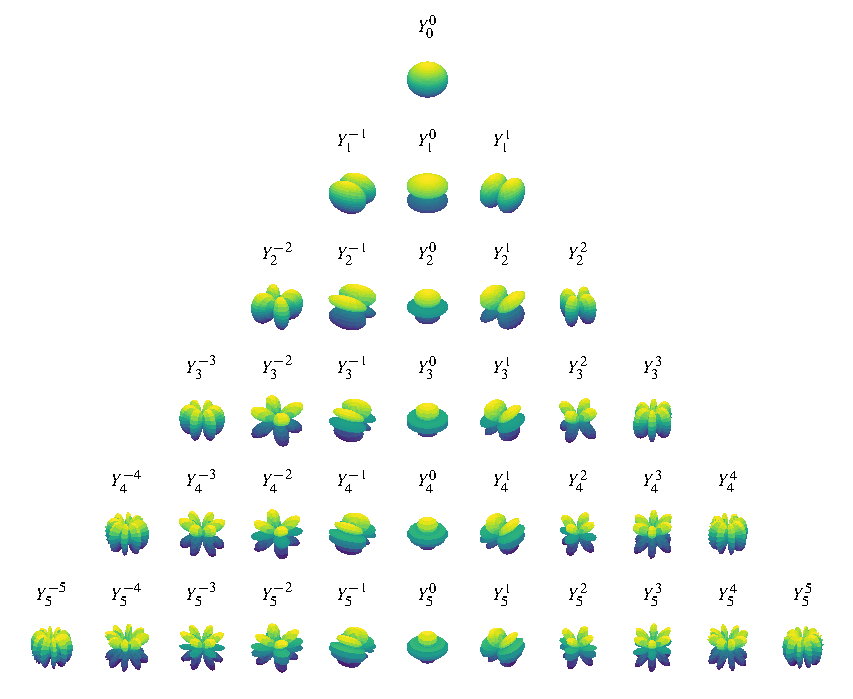
\includegraphics[width=\linewidth]{papers/kugel/figures/python/spherical-harmonics-triangle}
  \caption{
    \label{kugel:fig:spherical-harmonics}
    Spherical harmonics. The spherical harmonics are defined \emph{on} the
    surface of the sphere, however, for a more powerful visual intuition the
    radius was used to represent the real part of the function at each location
    on the unit sphere. 
    %
    % Since $\Re e^{im\varphi} = cos(m\varphi)$, $\Im e^{im\varphi} =
    % i\sin(m\varphi)$ and $\sin \alpha = \cos (\alpha - \pi/2)$, the imaginary
    % part has the same shape and is just ``rotated around the $z$ axis by
    % $\pi/2$''.
  }
\end{figure}
After this painful derivation, you would at least want to know how they look. 
Well, the figure \ref{kugel:fig:spherical-harmonics} serves precisely this 
purpose. 

The triangular style we used to represent them is quite evident. This arises 
naturally from the restriction we imposed on the indices $m,n$. Furthermore, 
because $Y^m_n$ are complex functions and we only have three dimensions 
available (visually), we decided to use the real part 
to show them, i.e. $\Re\left\{Y^m_n\right\}$.
\subsection{Orthogonality of $P_n$, $P^m_n$ and $Y^m_n$}
\label{kugel:sec:construction:orthogonality}

We shall now discuss an important property of the spherical harmonics: they form
an orthogonal system. And since the spherical harmonics contain the Ferrers or
associated Legendre functions, we need to discuss their orthogonality first.
But the Ferrers functions themselves depend on the Legendre polynomials, so that
will be our starting point.

\begin{lemma} For the Legendre polynomials $P_n(z)$ and $P_{n'}(z)$ it holds that
  \label{kugel:thm:legendre-poly-ortho}
  \begin{equation*}
    \int_{-1}^1 P_n(z) P_{n'}(z) \, dz
    = \frac{2}{2n + 1} \delta_{n'n}
    = \begin{cases}
      \frac{2}{2n + 1} & \text{if } n = {n'}, \\
      0 & \text{otherwise}.
    \end{cases}
  \end{equation*}
\end{lemma}
\begin{proof}
  To start, consider the fact that the Legendre equation
  \eqref{kugel:eqn:legendre}, of which two distinct Legendre polynomials
  $P_n(z)$ and $P_{n'}(z)$ are a solution ($n \neq {n'}$), can be rewritten in the
  following form:
  \begin{equation}
    \frac{d}{dz} \left[ 
      \left( 1 - z^2 \right) \frac{dZ}{dz}
    \right] + n(n+1) Z(z) = 0.
  \end{equation}
  So we rewrite the Legendre equations for $P_n(z)$ and $P_{n'}(z)$:
  \begin{align*}
    \frac{d}{dz} \left[ 
      \left( 1 - z^2 \right) \frac{dP_n}{dz}
    \right] + n(n+1) P_n(z) &= 0,
    &
    \frac{d}{dz} \left[ 
      \left( 1 - z^2 \right) \frac{dP_{n'}}{dz}
    \right] + {n'}({n'}+1) P_{n'}(z) &= 0,
  \end{align*}
  then we multiply the former by $P_{n'}(z)$ and the latter by $P_n(z)$ and
  subtract the two to get
  \begin{equation*}
    \frac{d}{dz} \left[ 
      \left( 1 - z^2 \right) \frac{dP_n}{dz}
    \right] P_{n'}(z) + n(n+1) P_n(z) P_{n'}(z)
    -
    \frac{d}{dz} \left[ 
      \left( 1 - z^2 \right) \frac{dP_{n'}}{dz}
    \right] P_n(z) - {n'}({n'}+1) P_{n'}(z) P_n(z) = 0.
  \end{equation*}
  By grouping terms, making order and integrating with respect to $z$ from $-1$
  to 1 we obtain
  \begin{gather}
    \int_{-1}^1 \left\{
      \frac{d}{dz} \left[ 
        \left( 1 - z^2 \right) \frac{dP_n}{dz}
      \right] P_{n'}(z) 
      -
      \frac{d}{dz} \left[ 
        \left( 1 - z^2 \right) \frac{dP_{n'}}{dz}
      \right] P_n(z) - {n'}({n'}+1) P_{n'}(z) P_n(z)
    \right\} \,dz \nonumber \\
    + \left[ n(n+1) - {n'}({n'}+1) \right] \int_{-1}^1 P_{n'}(z) P_n(z) \, dz = 0.
    \label{kugel:thm:legendre-poly-ortho:proof:1}
  \end{gather}
  Since by the product rule
  \begin{equation*}
    \frac{d}{dz} \left[ (1 - z^2) \frac{dP_{n'}}{dz} P_n(z) \right]
    =
    \frac{d}{dz} \left[ (1 - z^2) \frac{dP_n}{dz} \right] P_{n'}(z)
      + (1 - z^2) \frac{dP_n}{dz} \frac{dP_{n'}}{dz},
  \end{equation*}
  we can simplify the first term in
  \eqref{kugel:thm:legendre-poly-ortho:proof:1} to get
  \begin{gather*}
    \int_{-1}^1 \left\{
      \frac{d}{dz} \left[ (1 - z^2) \frac{dP_{n'}}{dz} P_n(z) \right]
        - \cancel{(1 - z^2) \frac{dP_n}{dz} \frac{dP_{n'}}{dz}}
        - \frac{d}{dz} \left[ (1 - z^2) \frac{dP_n}{dz} P_{n'}(z) \right]
        + \cancel{(1 - z^2) \frac{dP_{n'}}{dz} \frac{dP_n}{dz}}
    \right\} \, dz \\
    = \int_{-1}^1 \frac{d}{dz} \left\{ (1 - z^2) \left[
      \frac{dP_{n'}}{dz} P_n(z) - \frac{dP_n}{dz} P_{n'}(z)
    \right] \right\} \, dz
    = (1 - z^2) \left[
      \frac{dP_{n'}}{dz} P_n(z) - \frac{dP_n}{dz} P_{n'}(z)
    \right] \Bigg|_{-1}^1,
  \end{gather*}
  which always equals 0 because the product contains $1 - z^2$ and the bounds
  are at $\pm 1$. Thus, of \eqref{kugel:thm:legendre-poly-ortho:proof:1} only
  the second term remains and the equation becomes
  \begin{equation*}
    \left[ n(n+1) - {n'}({n'}+1) \right] \int_{-1}^1 P_{n'}(z) P_n(z) \, dz = 0.
  \end{equation*}
  By dividing by the constant in front of the integral we have our first result.
  Now we need to show that when $n = {n'}$ the integral equals $2 / (2n + 1)$.
  In order to achieve this, we will use what has now become our secret weapon: 
  integration by parts. We can start by rewriting the integral in the Lemma \label{kugel:thm:legendre-poly-ortho} for the case $n=n'$.
  According to Rodrigues formula, we have
  \begin{equation*}
    \int_{-1}^1 P_n(z)^2 dz = \left( \frac{1}{2^n n!} \right)^2 \int_{-1}^1 \frac{d^n}{dz^n} (z^2-1)^n \frac{d^n}{dz^n} (z^2-1)^n dz.
  \end{equation*}
  Now we can start the ``integration by parts process'', the first step would be
  \begin{align*}
    \int_{-1}^1 \frac{d^n}{dz^n} (z^2-1)^n \frac{d^n}{dz^n} (z^2-1)^n dz &= 
    \left[
      \frac{d^n}{dz^n} (z^2-1)^n \frac{d^{n-1}}{dz^{n-1}} (z^2-1)^n
    \right] \Bigg|_{-1}^1 \\
    &- \int_{-1}^1 \frac{d^{n+1}}{dz^{n+1}} (z^2-1)^n \frac{d^{n-1}}{dz^{n-1}} (z^2-1)^n dz \\
    &= - \int_{-1}^1 \frac{d^{n+1}}{dz^{n+1}} (z^2-1)^n \frac{d^{n-1}}{dz^{n-1}} (z^2-1)^n dz =: I_n.
  \end{align*}
  The reason why the first boundary-term vanishes is that we are dealing with a polynomial that has $n$ zeros at both boundary points. 
  By differentiating the latter $n-1$ times we will let these survive, making the whole term equal to zero. If we proceed with this process,
  the following equation can be inductively (and easily) derived
  \begin{equation*}
    I_n = (-1)^i \int_{-1}^1 \frac{d^{n+i}}{dz^{n+i}} (z^2-1)^n \frac{d^{n-i}}{dz^{n-i}} (z^2-1)^n dz, \quad i \in \mathbb{N}_0.
  \end{equation*}
  By letting $i=n$, we arrive at
  \begin{equation*}
    I_n = (-1)^n \int_{-1}^1 \frac{d^{2n}}{dz^{2n}} (z^2-1)^n (z^2-1)^n dz = (-1)^n (2n)! \int_{-1}^1 (z^2-1)^n dz.
  \end{equation*}
  The new problem is now to compute the integral of $(z^2-1)^n$. To go further we can once again use integration by parts, obtaining
  \begin{align*}
    \int_{-1}^1 (z^2-1)^n dz =  \left[
       z(z^2-1)^n
      \right] \Bigg|_{-1}^1 -2n \int_{-1}^1 z^2 (z^2-1)^{n-1} dz 
      &= -2n \int_{-1}^1 (z^2-1+1) (z^2-1)^{n-1} dz \\
      &= -2n \int_{-1}^1 (z^2-1)^n + (z^2-1)^{n-1} dz.
  \end{align*}
  Now, by multiplying both sides by $(-1)^n(2n)!$, we can express the last equation in terms of $I_n$, namely
  \begin{equation}
    I_n = -2n ( I_n + I_{n-1} ) \iff I_n = -\frac{2n}{2n+1} I_{n-1}. \label{kugel:eq:recursion_proof}
  \end{equation}
  We can hence rewrite eq.\eqref{kugel:eq:recursion_proof} as
  \begin{align*}
    I_n &= \frac{2n}{2n+1} \frac{2(n-1)}{2(n-1)+1} I_{n-2} = (-1)^n \frac{2n \cdot \hdots \cdot 6\cdot 4\cdot 2}{(2n+1) \cdot \hdots \cdot 7 \cdot 5 \cdot 3} I_0 \\
        &= (-1)^n \frac{(2n \cdot \hdots \cdot 6\cdot 4\cdot 2)(2n \cdot \hdots \cdot 6\cdot 4\cdot 2)}
                       {(2n+1)(2n)\cdot \hdots \cdot 7\cdot 6\cdot 5\cdot 4\cdot 3\cdot 2} I_0 = (-1)^n \frac{2^{2n}(n\cdot \hdots \cdot 3 \cdot 2 \cdot 1)^2}
                                                                                                             {(2n+1)!} I_0 \\
    &= (-1)^n  \frac{2^{2n}(n!)^2}{(2n+1)!} I_0 .
  \end{align*}
  The only thing left to know is $I_0$, that can be trivially obtained using the definition of $I_n$. We can write
  \begin{equation*}
    I_0 = (-1)^n(2n)! \int_{-1}^1 (1-z^2)^0 dz = (-1)^n(2n)! 2,
  \end{equation*}
  meaning that
  \begin{equation*}
    I_n = (-1)^n  \frac{2^{2n}(n!)^2}{(2n+1)!} \cdot (-1)^n(2n)! 2
  \end{equation*}
  and consequently
  \begin{equation*}
      \int_{-1}^1 P_n(z)^2 dz = \left( \frac{1}{2^n n!} \right)^2 \cdot (-1)^n  \frac{2^{2n}(n!)^2}{(2n+1)!} \cdot (-1)^n(2n)! 2 = \frac{2}{2n+1}.
  \end{equation*}

\end{proof}

In a similarly algebraically tedious fashion, we can also continue to check for
orthogonality for the Ferrers functions $P^m_n(z)$, since they are related to
$P_n(z)$ by a $m$-th derivative, and obtain the following result.

\begin{lemma} For the associated Legendre functions
  \label{kugel:thm:associated-legendre-ortho}
  \begin{equation*}
    \int_{-1}^1 P^m_n(z) P^{m}_{n'}(z) \, dz
    = \frac{2(m + n)!}{(2n + 1)(n - m)!} \delta_{nn'}
    = \begin{cases}
      \frac{2(m + n)!}{(2n + 1)(n - m)!}
        & \text{if } n = n', \\
      0 & \text{otherwise}.
    \end{cases}
  \end{equation*}
\end{lemma}
\begin{proof}
  To show that the expression equals zero when $n \neq n'$ we can perform
  exactly the same steps as in the proof of lemma
  \ref{kugel:thm:legendre-poly-ortho}, so we will not repeat them here.
\end{proof}

By having the orthogonality relations of the Legendre functions we can finally
show that spherical harmonics are also orthogonal under the following inner
product:

\begin{definition}[Inner product in $S^2$]
  \label{kugel:def:inner-product-s2}
  For two complex valued functions $f(\vartheta, \varphi)$ and $g(\vartheta,
  \varphi)$ on the surface of the sphere the inner product is defined to be
  \begin{equation*}
    \langle f, g \rangle
    = \int_{0}^\pi \int_0^{2\pi}
      f(\vartheta, \varphi) \overline{g(\vartheta, \varphi)}
      \sin \vartheta \, d\varphi \, d\vartheta.
  \end{equation*}
\end{definition}


\begin{theorem} For the (unnormalized) spherical harmonics
  \label{kugel:thm:spherical-harmonics-ortho}
  \begin{align}
    \langle Y^m_n, Y^{m'}_{n'} \rangle
    &= \int_{0}^\pi \int_0^{2\pi}
      Y^m_n(\vartheta, \varphi) \overline{Y^{m'}_{n'}(\vartheta, \varphi)}
      \sin \vartheta \, d\varphi \, d\vartheta
      \label{kugel:eq:spherical-harmonics-inner-prod} \\
    &= \frac{4\pi}{2n + 1} \frac{(m + n)!}{(n - m)!} \delta_{nn'} \delta_{mm'}
    = \begin{cases}
      \frac{4\pi}{2n + 1} \frac{(m + n)!}{(n - m)!}
        & \text{if } n = n' \text{ and } m = m', \nonumber \\
      0 & \text{otherwise}.
    \end{cases}
  \end{align}
\end{theorem}
\begin{proof}
  We will begin by doing a bit of algebraic manipulation \footnote{
    Essentially, what we just did was to turn
    \eqref{kugel:eq:spherical-harmonics-inner-prod} in this form:
    \(
      \langle Y^m_n, Y^{m'}_{n'} \rangle_{\partial S}
      = \langle P^m_n, P^{m'}_{n'} \rangle_z
      \; \langle e^{im\varphi}, e^{-im'\varphi} \rangle_\varphi
    \).
  }:
  \begin{align*}
    \int_{0}^\pi \int_0^{2\pi}
      Y^m_n(\vartheta, \varphi) \overline{Y^{m'}_{n'}(\vartheta, \varphi)} 
      \sin \vartheta \, d\varphi \, d\vartheta
    &= \int_{0}^\pi \int_0^{2\pi}
      e^{im\varphi} P^m_n(\cos \vartheta)
      e^{-im'\varphi} P^{m'}_{n'}(\cos \vartheta)
      \, d\varphi \sin \vartheta \, d\vartheta 
    \\
    &= \int_{0}^\pi
      P^m_n(\cos \vartheta) P^{m'}_{n'}(\cos \vartheta) \sin \vartheta \, d\vartheta
      \int_0^{2\pi} e^{i(m - m')\varphi}
      \, d\varphi. 
  \end{align*}
  First, notice that the associated Legendre polynomials are assumed to be real,
  and are thus unaffected by the complex conjugation. Then, we can see that when
  $m = m'$ the inner integral simplifies to $\int_0^{2\pi} 1 \, d\varphi$ which
  equals $2\pi$, so in this case the expression becomes
  \begin{equation*}
    2\pi \int_{0}^\pi
      P^m_n(\cos \vartheta) P^{m'}_{n'}(\cos \vartheta)
    \sin \vartheta \, d\vartheta
    = -2\pi \int_{1}^{-1} P^m_n(z) P^{m'}_{n'}(z) \, dz
    = \frac{4\pi(m + n)!}{(2n + 1)(n - m)!} \delta_{nn'},
  \end{equation*}
  where in the second step we performed the substitution $z = \cos\vartheta$;
  $d\vartheta = \frac{d\vartheta}{dz} dz= - dz / \sin \vartheta$, and then we
  used lemma \ref{kugel:thm:associated-legendre-ortho}.  We are allowed to use
  the lemma because $m = m'$. Now we just need look at the case when $m \neq
  m'$. Fortunately this is easier: the inner integral is $\int_0^{2\pi} e^{i(m -
  m')\varphi} d\varphi$, or in other words we are integrating a complex
  exponential over the entire period, which always results in zero. Thus, we do
  not need to do anything and the proof is complete.
\end{proof}

These proofs for the various orthogonality relations were quite long and
algebraically tedious, mainly because they are ``low level'', by which we mean
that they (arguably) do not rely on very abstract theory. However, if we allow
ourselves to use the more abstract Sturm Liouville theory discussed in section
\ref{buch:integrale:subsection:sturm-liouville-problem} and chapter
\ref{chapter:sturmliouville} the proofs can become ridiculously short. Let's do
for example lemma \ref{kugel:thm:associated-legendre-ortho}.

\begin{proof}[Shorter proof of lemma 
  \ref{kugel:thm:associated-legendre-ortho}]
  The associated Legendre polynomials, of which we would like to prove an
  orthogonality relation, are the solution to the associated Legendre equation,
  which we can write as $LZ(z) = 0$, where
  \begin{equation*}
    L = \frac{d}{dz} (1 - z^2) \frac{d}{dz}
      + n(n+1) - \frac{m^2}{1 - z^2}.
  \end{equation*}
  Notice that $L$ is in fact a Sturm-Liouville operator of the form
  \begin{equation*}
    L = \frac{1}{w(z)} \left[
        \frac{d}{dz} p(z) \frac{d}{dz} - \lambda + q(z)
      \right],
  \end{equation*}
  if we let $w(z) = 1$, $p(z) = (1 - z^2 )$, $q(z) = -m^2 / (1 - z^2)$, and
  $\lambda = -n(n+1)$. By the theory of Sturm-Liouville operators, we know that
  the each solution of the problem $LZ(z) = 0$, namely $P^m_n(z)$, is orthogonal
  to every other solution that has a different $\lambda$. In our case $\lambda$
  varies with $n$, so $P^m_n(z)$ with different $n$'s are orthogonal to each
  other.
\end{proof}

But that was still rather informative and had a bit of explanation, which is
terrible. Real snobs, such as Wikipedia contributors, some authors and
regrettably sometimes even ourselves, would write instead:

\begin{proof}[Infuriatingly short proof of lemma
  \ref{kugel:thm:associated-legendre-ortho}]
  The associated Legendre polynomials are solutions of the associated Legendre
  equation which is a Sturm-Liouville problem and are thus orthogonal to each
  other. The factor in front Kronecker delta is left as an exercise to the
  reader.
\end{proof}

Lemma \ref{kugel:thm:legendre-poly-ortho} has a very similar proof, while
theorem \ref{kugel:thm:spherical-harmonics-ortho} for the spherical harmonics is
proved by the following argument.  The spherical harmonics are the solutions to
the eigenvalue problem $\surflaplacian f = -\lambda f$, which as discussed in
the previous section is solved using the separation Ansatz. So to prove their
orthogonality using the Sturm-Liouville theory we argue that
\begin{equation*}
  \surflaplacian = L_\vartheta L_\varphi \iff
  \surflaplacian f(\vartheta, \varphi)
    = L_\vartheta \Theta(\vartheta) L_\varphi \Phi(\varphi),
\end{equation*}
then we show that both $L_\vartheta$ and $L_\varphi$ are both Sturm-Liouville
operators (we just did the former in the shorter proof above). Since both are
Sturm-Liouville operators their combination, the surface spherical Laplacian, is
also a Sturm-Liouville operator, which then implies orthogonality.

\subsection{Normalization and the Phase Factor}

At this point we have shown that the spherical harmonics form an orthogonal
system, but in many applications we usually also want a normalization of some
kind. For example the most obvious desirable property could be for the spherical
harmonics to be ortho\emph{normal}, by which we mean that $\langle Y^m_n,
Y^{m'}_{n'} \rangle = \delta_{nn'} \delta_{mm'}$. To obtain orthonormality, we
simply add an ugly normalization factor in front of the previous definition
\ref{kugel:def:spherical-harmonics} as follows.

\begin{definition}[Orthonormal spherical harmonics]
  \label{kugel:def:spherical-harmonics-orthonormal}
  The functions
  \begin{equation*}
    Y^m_n(\vartheta, \varphi)
    = \sqrt{\frac{2n + 1}{4\pi} \frac{(n-m)!}{(m+n)!}}
      P^m_n(\cos \vartheta) e^{im\varphi}
  \end{equation*}
  where $m, n \in \mathbb{Z}$ and $|m| < n$ are the orthonormal spherical
  harmonics.
\end{definition}

Orthornomality is very useful, but it is not the only common normalization that
is found in the literature. In physics, geomagnetism to be more specific, it is
common to use the so called Schmidt semi-normalization (or sometimes also called
quasi-normalization).

\begin{definition}[Schmidt semi-normalized spherical harmonics]
  \label{kugel:def:spherical-harmonics-schmidt}
  The Schmidt semi-normalized spherical harmonics are
  \begin{equation*}
    Y^m_n(\vartheta, \varphi)
    = \sqrt{2 \frac{(n - m)!}{(n + m)!}}
      P^m_n(\cos \vartheta) e^{im\varphi}
  \end{equation*}
  where $m, n \in \mathbb{Z}$ and $|m| < n$.
\end{definition}

Additionally, there is another quirk in the literature that should be mentioned.
In some other branches of physics such as seismology and quantum mechanics there
is a so called Condon-Shortley phase factor $(-1)^m$ in front of the square root
in the definition of the normalized spherical harmonics. It is yet another
normalization that is added for physical reasons that are not very relevant to
our discussion, but we mention this potential source of confusion since many
numerical packages (such as \texttt{SHTOOLS}
\cite{markwieczorek_shtoolsshtools_2022}) offer an option to add or remove it
from the computation.

Though, for our purposes we will mostly only need the orthonormal spherical
harmonics, so from now on, unless specified otherwise when we say spherical
harmonics or write $Y^m_n$, we mean the orthonormal spherical harmonics of
definition \ref{kugel:def:spherical-harmonics-orthonormal}.

\subsection{Recurrence Relations}
\label{kugel:sec:construction:recurrence}

The idea of this subsection is to introduce first some recursive relations
regarding the associated Legendre functions, defined in equation
\eqref{kugel:def:ferrers-functions}. Subsequently we will extend them, in order
to derive recurrence formulas for the case of spherical harmonic functions as
well.

\subsubsection{Associated Legendre Functions}

To start this journey, we can first write the following equations, which relate
the associated Legendre functions of different indices $m$ and $n$ recursively:
\begin{subequations}
  \begin{align}
    P^m_n(z) &= \dfrac{1}{(2n+1)z} \left[
       (m+n) P^m_{n-1}(z) + (n-m+1) P^m_{n+1}(z)
     \right] \label{kugel:eqn:rec-leg-1} \\
    P^m_n(z) &= \dfrac{\sqrt{1-z^2}}{2mz} \left[
        P^{m+1}_n(z) + [n(n+1)-m(m-1)] P^{m-1}_n(z)
      \right] \label{kugel:eqn:rec-leg-2} \\ 
    P^m_n(z) &= \dfrac{1}{(2n+1)\sqrt{1-z^2}} \left[
        P^{m+1}_{n+1}(z) - P^{m+1}_{n-1}(z)
      \right] \label{kugel:eqn:rec-leg-3} \\
    P^m_n(z) &= \dfrac{1}{(2n+1)\sqrt{1-z^2}} \left[
        (n+m)(n+m-1)P^{m-1}_{n-1}(z) - (n-m+1)(n-m+2)P^{m-1}_{n+1}(z)
      \right] \label{kugel:eqn:rec-leg-4}
  \end{align}
\end{subequations}

Much of the effort will be proving this bunch of equalities. Then, in the second
part, where we will derive the recursion equations for
$Y^m_n(\vartheta,\varphi)$, we will basically reuse the ones presented above.
Maybe it is worth mentioning at least one use case for these relations: In some
software implementations (that include lighting computations in computer
graphics, antenna modelling software, 3D modelling in medical applications,
etc.) they are widely used, as they lead to better numerical accuracy and
computational cost lower by a factor of six \cite{davari_new_2013}.

\begin{proof}[Proof of \eqref{kugel:eqn:rec-leg-1}]
  This is the relation that links the associated Legendre functions with the
  same $m$ index but different $n$. Using theorem
  \ref{buch:orthogonal:satz:drei-term-rekursion}, we have 
  \begin{equation*}
    (n+1)P_{n+1}(z)-(2n+1)zP_n(z)+nP_{n-1}(z)=0,
  \end{equation*}
  that can be differentiated $m$ times, obtaining
  \begin{equation}
    \label{kugel:eq:rec_1}
    (n+1)\frac{d^mP_{n+1}}{dz^m}-(2n+1) \left[
      z \frac{d^m P_n}{dz^m}+ m\frac{d^{m-1}P_{n-1}}{dz^{m-1}}
    \right] + n\frac{d^m P_{n-1}}{dz^m} = 0.
  \end{equation}
  To continue this derivation, we need the following relation:
  \begin{equation}
    \label{kugel:eq:rec_2}
    \frac{dP_{n+1}}{dz} - \frac{dP_{n-1}}{dz} = (2n+1)P_n.
  \end{equation}
  The latter will not be derived, because it suffices to use the definition of
  the Legendre polynomials $P_n(z)$ to check it.  We can now differentiate $m-1$
  times the just presented equation \eqref{kugel:eq:rec_2}, that so that is
  becomes
  \begin{equation}
    \label{kugel:eq:rec_3}
    \frac{d^mP_{n+1}}{dz^m} - \frac{d^mP_{n-1}}{dz^m}
    = (2n+1)\frac{d^{m-1}P_n}{dz^{m-1}}.
  \end{equation}
  Then, using \eqref{kugel:eq:rec_3} in \eqref{kugel:eq:rec_1}, we will
  have
  \begin{equation}
    \label{kugel:eq:rec_4}
    (n+1)\frac{d^mP_{n+1}}{dz^m}
      - (2n+1)\frac{d^mP_{n+1}}{dz^m}
      - m\left[\frac{d^m P_{n+1}}{dz^m}
      + \frac{d^{m}P_{n-1}}{dz^m}\right]
      + n\frac{d^m P_{n-1}}{dz^m}=0.
  \end{equation}
  Finally, multiplying both sides by $(1-z^2)^{\frac{m}{2}}$ and simplifying the
  expression, we can rewrite \eqref{kugel:eq:rec_4} in terms of $P^m_n(z)$,
  namely
  \begin{equation*}
    (n+1-m)P^m_{n+1}(z)-(2n+1)zP^m_n(z)+(m+n)P^m_{n-1}(z)=0,
  \end{equation*}
  that rearranged, will be
  \begin{equation*}
    (2n+1) z P^m_n(z)= (m+n) P^m_{n-1}(z) + (n-m+1) P^m_{n+1}(z).
    \qedhere
  \end{equation*}
\end{proof}

\begin{proof}[Proof of \eqref{kugel:eqn:rec-leg-2}]
  This relation, unlike the previous one, links three expressions with the same
  $n$ index but different $m$. In the proof of lemma
  \ref{kugel:thm:extend-legendre}, at some point we ran into this expression.
  \begin{equation*}
    (1-z^2)\frac{d^{m+2}P_n}{dz^{m+2}}
    - 2(m+1)z \frac{d^{m+1}P_n}{dz^{m+1}}
    + [n(n+1)-m(m+1)]\frac{d^mP_n}{dz^m} = 0,
  \end{equation*}
  which, if multiplied by $(1-z^2)^{\frac{m}{2}}$, becomes
  \begin{equation*}
    (1-z^2)^{\frac{m}{2}+1}\frac{d^{m+2}P_n}{dz^{m+2}}
    - 2(m+1)z (1-z^2)^{\frac{m}{2}}\frac{d^{m+1}P_n}{dz^{m+1}}
    + [n(n+1)-m(m+1)](1-z^2)^{\frac{m}{2}}\frac{d^mP_n}{dz^m} = 0.
  \end{equation*}
  Therefore, as before, expressing it in terms of $P^m_n(z)$:
  \begin{equation*}
    P^{m+2}_n(z) - \frac{2(m+1)z}{\sqrt{1-z^2}}P^{m+1}_n(z)
    + [n(n+1)-m(m+1)]P^m_n(z)=0.
  \end{equation*}
  Further, we can adjust the indices and terms, obtaining
  \begin{equation*}
    \frac{2mz}{\sqrt{(1-z^2)}} P^m_n(z)
    = P^{m+1}_n(z) + [n(n+1)-m(m-1)] P^{m-1}_n(z).
    \qedhere
  \end{equation*}
\end{proof}

\begin{proof}[Proof of \eqref{kugel:eqn:rec-leg-3}]
  To derive this expression, we can multiply \eqref{kugel:eq:rec_3} by
  $(1-z^2)^{\frac{m}{2}}$ and, as always, we could express it in terms of
  $P^m_n(z)$:
  \begin{equation*}
    P^m_{n+1}(z) - P^m_{n-1}(z) = (2n+1)\sqrt{1-z^2}P^{m-1}_n(z).
  \end{equation*}
  After that we can divide by $2n+1$ resulting in
  \begin{equation}\label{kugel:eq:helper}
    \frac{1}{2n+1}[P^m_{n+1}(z) - P^m_{n-1}(z)] = \sqrt{1-z^2}P^{m-1}_n(z).
  \end{equation}
  To conclude, we arrange the indices differently:
  \begin{equation*}
    \sqrt{1-z^2}P^{m}_n(z)=\frac{1}{2n+1}[P^{m+1}_{n+1}(z) - P^{m+1}_{n-1}(z)].
    \qedhere
  \end{equation*}
\end{proof}

\begin{proof}[Proof of \eqref{kugel:eqn:rec-leg-4}]
  For this proof we can rely on \eqref{kugel:eqn:rec-leg-1}, and therefore
  rewrite \eqref{kugel:eqn:rec-leg-2} as 
  \begin{equation*}
    \frac{2m}{(2n+1)\sqrt{1-z^2}} \left[
      (m+n)P^m_{n-1}(z) + (n-m+1)P^m_{n+1}(z)
    \right] = P^{m+1}_n(z) + [ n(n+1)-m(m-1) ]P^{m-1}_n(z).
  \end{equation*}
  Rewriting then $P^{m-1}_n(z)$ using \eqref{kugel:eq:helper}, we will have
  \begin{align*}
    \frac{2m}{(2n+1)\sqrt{1-z^2}}
      &\left[ (m+n)P^m_{n-1}(z) + (n-m+1)P^m_{n+1}(z) \right] = P^{m+1}_n(z) \\
      &+ \frac{n(n+1)-m(m-1)}{(2n+1)\sqrt{1-z^2}} \left[
          P^m_{n+1}(z)-P^m_{n-1}(z)
        \right].
  \end{align*}
  The last equation, after some algebraic rearrangements, it is easy to show
  that it is equivalent to
  \begin{equation*}
    \sqrt{1-z^2} P^m_n(z) = \dfrac{1}{2n+1} \left[
      (n+m)(n+m-1)P^{m-1}_{n-1}(z) - (n-m+1)(n-m+2)P^{m-1}_{n+1}(z)
    \right].
    \qedhere
  \end{equation*}
\end{proof}

\subsubsection{Spherical Harmonics}

The goal of this subsection's part is to apply the recurrence relations of the
$P^m_n(z)$ functions to the spherical harmonics.  With some little adjustments
we will be able to have recursion equations for them too. As previously written
most of the work is already done. Now it is only a matter of minor mathematical
operations/rearrangements. We can start by listing all of them:
\begin{subequations}
  \begin{align}
  Y^m_n(\vartheta, \varphi) &= \dfrac{1}{(2n+1)\cos \vartheta} \left[
      (m+n)Y^m_{n-1}(\vartheta, \varphi)
      + (m-n+1)Y^m_{n+1}(\vartheta, \varphi)
    \right] \label{kugel:eqn:rec-sph-harm-1} \\
  Y^m_n(\vartheta, \varphi) &= \dfrac{\tan \vartheta}{2m}\left[
      Y^{m+1}_n(\vartheta, \varphi)e^{-i\varphi}
      + [n(n+1)-m(m-1)]Y^{m-1}_n(\vartheta, \varphi)e^{i\varphi}
    \right] \label{kugel:eqn:rec-sph-harm-2} \\
  Y^m_n(\vartheta, \varphi) &= \dfrac{e^{-i\varphi}}{ (2n+1)\sin \vartheta}
    \left[
      Y^{m+1}_{n+1}(\vartheta, \varphi)
      - Y^{m+1}_{n-1}(\vartheta, \varphi)
    \right] \label{kugel:eqn:rec-sph-harm-3} \\
  Y^m_n(\vartheta, \varphi) &= \dfrac{e^{i\varphi}}{(2n+1)\sin \vartheta}
    \left[
      (n+m)(n+m-1)Y^{m-1}_{n-1}(\vartheta, \varphi)
      - (n-m+1)(n-m+2)Y^{m-1}_{n+1}(\vartheta, \varphi)
    \right] \label{kugel:eqn:rec-sph-harm-4} 
  \end{align}
\end{subequations}

\begin{proof}[Proof of \eqref{kugel:eqn:rec-sph-harm-1}]
  We can multiply both sides of equality in \eqref{kugel:eqn:rec-leg-1} by $e^{im
  \varphi}$ and perform the substitution $z=\cos \vartheta$. After a few simple
  algebraic steps, we will obtain the relation we are looking for.
\end{proof}

\begin{proof}[Proof of \eqref{kugel:eqn:rec-sph-harm-2}]
  In this proof, as before, we can perform the substitution $z=\cos \vartheta$,
  and notice that $\sqrt{1-z^2}=\sin \vartheta$, hence, the relation in
  \eqref{kugel:eqn:rec-leg-2} will be
  \begin{equation*}
    \frac{2m \cos \vartheta}{\sin \vartheta} P^m_n(\cos \vartheta) 
    = P^{m+1}_n(\cos \vartheta) + [n(n+1)-m(m-1)]P^{m-1}_n P^m_n(\cos \vartheta).
  \end{equation*}
  The latter, multiplied by $e^{im\varphi}$, becomes
  \begin{align*}
    \frac{2m \cos \vartheta}{\sin \vartheta} P^m_n(\cos \vartheta)e^{im\varphi}
      &= P^{m+1}_n(\cos \vartheta)e^{im\varphi}
       + [n(n+1)-m(m-1)]P^{m-1}_n P^m_n(\cos \vartheta)e^{im\varphi} \\
      &= P^{m+1}_n(\cos \vartheta)e^{i(m+1)\varphi}e^{-i\varphi}
       + [n(n+1)-m(m-1)]P^{m-1}_n (\cos \vartheta)e^{i(m-1)\varphi}e^{i\varphi} \\
      &= Y^{m+1}_n(\vartheta, \varphi)e^{-i\varphi}
       + [n(n+1)-m(m-1)]Y^{m-1}_n(\vartheta, \varphi)e^{i\varphi}.
  \end{align*}
  Finally, after some ``cleaning''
  \begin{equation*}
    Y^m_n(\vartheta, \varphi) = \frac{\tan \vartheta}{2m} \left[
      Y^{m+1}_n(\vartheta, \varphi)e^{-i\varphi}
      + [n(n+1)-m(m-1)]Y^{m-1}_n(\vartheta, \varphi)e^{i\varphi}
    \right]
    \qedhere
  \end{equation*}
\end{proof}

\begin{proof}[Proof of \eqref{kugel:eqn:rec-sph-harm-3}]
  Now we can consider \eqref{kugel:eqn:rec-leg-3}, and multiply it by
  $e^{im\varphi}$. After the usual substitution $z=\cos \vartheta$, we have 
  \begin{align*}
    \sin \vartheta P^m_n(\cos \vartheta)e^{im\varphi}
      &= \dfrac{e^{im\varphi}}{2n+1}\left[
          P^{m+1}_{n+1}(\cos \vartheta)
          - P^{m+1}_{n-1}(\cos \vartheta)
        \right] \\
      &= \dfrac{e^{-i\varphi}}{2n+1}\left[
          P^{m+1}_{n+1}(\cos \vartheta)e^{i(m+1)\varphi}
          - P^{m+1}_{n-1}(\cos \vartheta)e^{i(m+1)\varphi}
        \right].
  \end{align*}
  A few manipulations later, we will obtain
  \begin{equation*}
    Y^m_n(\vartheta, \varphi) = \frac{e^{-i\varphi}}{(2n+1)\sin \vartheta}
      \left[
        Y^{m+1}_{n+1}(\vartheta, \varphi)-Y^{m+1}_{n-1}(\vartheta, \varphi)
      \right].
    \qedhere
  \end{equation*}
\end{proof}

\begin{proof}[Proof of \eqref{kugel:eqn:rec-sph-harm-4}]
  This proof is very similar to the previous one. We just have to perform the
  substitution $z = \cos \vartheta$, as always. Secondly we can multiply the
  right side by $e^{im\varphi}$ and the left one too but in a different form,
  namely $e^{im\varphi}=e^{i(m-1)\varphi}e^{i\varphi}$. Then it is only a
  question of recalling the definition of $Y^m_n(\vartheta, \varphi)$.
\end{proof}

\section{Series Expansions in $L^2(S^2)$}
\label{kugel:sec:expansion}
\kopfrechts{Series Expansions in $L^2(S^2)$}

We have now reached a point where we have all the tools that are necessary to
build something truly amazing: a general series expansion formula for function
on the surface of the sphere.  Before starting we want to recall the definition
of the inner product on the spherical surface of definition
\ref{kugel:def:inner-product-s2}
\begin{equation*}
  \langle f, g \rangle
  = \int_{0}^\pi \int_0^{2\pi}
    f(\vartheta, \varphi) \overline{g(\vartheta, \varphi)}
    \sin \vartheta \, d\varphi \, d\vartheta.
\end{equation*}
To be a bit technical we can say that the set of spherical harmonic functions,
together with the inner product just showed, form a Hilbert space. This function
space is defined over the space of ``well-behaved''\footnote{The definition of
``well-behaved'' is pretty ambiguous even for mathematicians, basically, it
depends on the context. We can cheat by saying: functions for which the theory
we are considering (Fourier theorem) is valid.} functions.  We can say that the
theory we are about to show can be applied on all twice differentiable complex
valued functions, to be more concise: complex valued $L^2$ functions $S^2 \to
\mathbb{C}$. However, all of this jargon is not really necessary for the
practical applications of us mere mortals, namely physicists and engineers.
From now on we will therefore assume that the functions we will dealing with
fulfill these ``minor'' conditions.

The insiders could turn up their nose, but we don't want to dwell too much on
the concept of Hilbert space, convergence, metric, well-behaved functions etc.
We simply think that too much rigorousness would be at the expense of the
possibility to appreciate the beauty and elegance of this theory.  Furthermore,
the risk of writing over 300 pages to prove that $1+1=2$ is just around the
corner (we apologize to Mr. Whitehead and Mr. Russel for using their efforts
\cite{principia-mathematica} with a negative connotation).

\subsection{Spherical Harmonics Series}

To talk about a series expansion we first need a \emph{series}, so we shall
build one using the spherical harmonics.

\begin{definition}[Spherical harmonic series]
  \label{kugel:def:spherical-harmonics-series}
  \begin{equation}
    \label{kugel:eqn:spherical-harmonics-series}
    f(\vartheta, \varphi) 
    = \sum_{n=0}^\infty \sum_{m =-n}^n
      c_{m,n} Y^m_n(\vartheta, \varphi).
  \end{equation}
\end{definition}

With this definition of course we are hinting that any function defined on the
spherical surface can be represented as a linear combination of spherical
harmonics. So, does \eqref{kugel:eqn:spherical-harmonics-series} sound familiar?
It should, since this is analog to the classical Fourier theory of section
\ref{kugel:sec:preliminaries:ortho-fourier} were it was stated that ``any''
1-periodic function $f(\xi, \eta)$, can be represented as a linear combination
of complex exponentials:
\begin{equation*}
  f(\xi, \eta) = \sum_{n \in \mathbb{Z}} \sum_{m \in \mathbb{Z}}
    c_{m,n} e^{i2\pi(n\xi + m\eta)},
\end{equation*}
In definition \ref{kugel:def:spherical-harmonics-series} it is the same, except
that the kernels are the spherical harmonics $Y^m_n$ instead of complex
exponentials. Further, as in the normal Fourier theory if we assume that a
function on the surface of the sphere can be represented using a Fourier series
we can use the same trick with the inner product to get the coefficients:
\begin{align*}
  \langle f, Y^{m}_{n} \rangle_{\partial S}
  = \left\langle \sum_{n'=0}^\infty \sum_{m' =-n'}^{n'}
    c_{m',n'} Y^{m'}_{n'}(\vartheta, \varphi), Y^{m}_{n} 
    \right\rangle_{\partial S}
  % &=  \sum_{n'=0}^\infty \sum_{m' =-n'}^{n'}
  %   \langle c_{m',n'} Y^{m'}_{n'}, Y^{m}_{n} \rangle_{\partial S}
  = \sum_{n'=0}^\infty \sum_{m' =-n'}^{n'} c_{m',n'}
    \langle Y^{m'}_{n'}, Y^{m}_{n} \rangle_{\partial S} = c_{m,n}.
\end{align*}

Finally, it can also be shown that for the famous ``well-behaved functions''
mentioned before, the following theorem is true. The connection to theorem
\ref{kugel:thm:fourier-theorem} is pretty obvious.

\begin{theorem}[Fourier theorem on $\partial S$]
  \label{kugel:thm:fourier-s2}
  For a function $f: S^2 \to \mathbb{C}$ and such that $f \in L^2$
  \begin{equation*}
    \lim_{N \to \infty}
    \biggl\|
      f(\vartheta,\varphi)
      - \sum_{n=0}^N\sum_{m=-n}^n c_{m,n} Y^m_n(\vartheta,\varphi)
    \biggr\|_2 = 0,
    \qquad\text{where}\qquad
    c_{m,n} = \langle f, Y^m_n \rangle.
  \end{equation*}
\end{theorem}
\begin{proof}
  Fourier was quite informal the first time he presented his theorem so, like
  him, we will just say ``trust me, it works''. In any case, for the ones that
  are brave enough and want a real proof, Dirichlet et al. can help with the
  case in one dimension \cite{convergence_fourier}.
\end{proof}

\subsection{Spectrum}
\label{kugel:sec:spectrum}

\begin{figure}
  \centering
  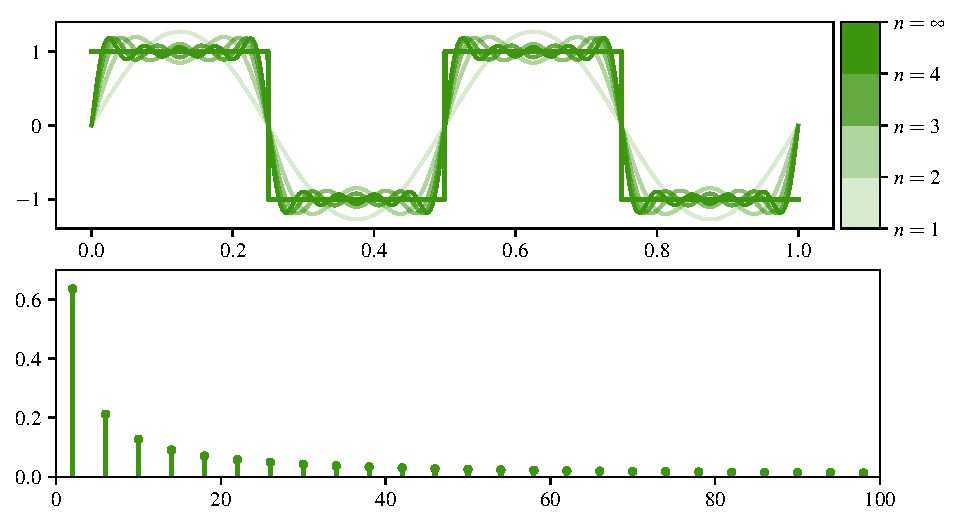
\includegraphics[width=.95\textwidth]{papers/kugel/figures/python/1D-fourier.pdf}
  \caption{
    Square signal (above) with the magnitude squared of its respective Fourier
    coefficients $c_n$, that are given by $c_{2n+1}=\frac{2}{i\pi(2n+1)}$. The
    graphic above also shows different reconstructions of the signal $y(x)$ with
    increasing $n$.
    \label{kugel:fig:1d-fourier}
  }
\end{figure}

 In the case of the classical one dimensional Fourier theory, in the most
 general case the \emph{spectrum} $c_n$ are complex numbers, so we divide the
 concept of spectrum in \emph{amplitude spectrum} and \emph{phase spectrum}. In
 figure \ref{kugel:fig:1d-fourier} a function $f(x)$ is presented along with the
 amplitude spectrum.

\begin{figure}
  \centering
  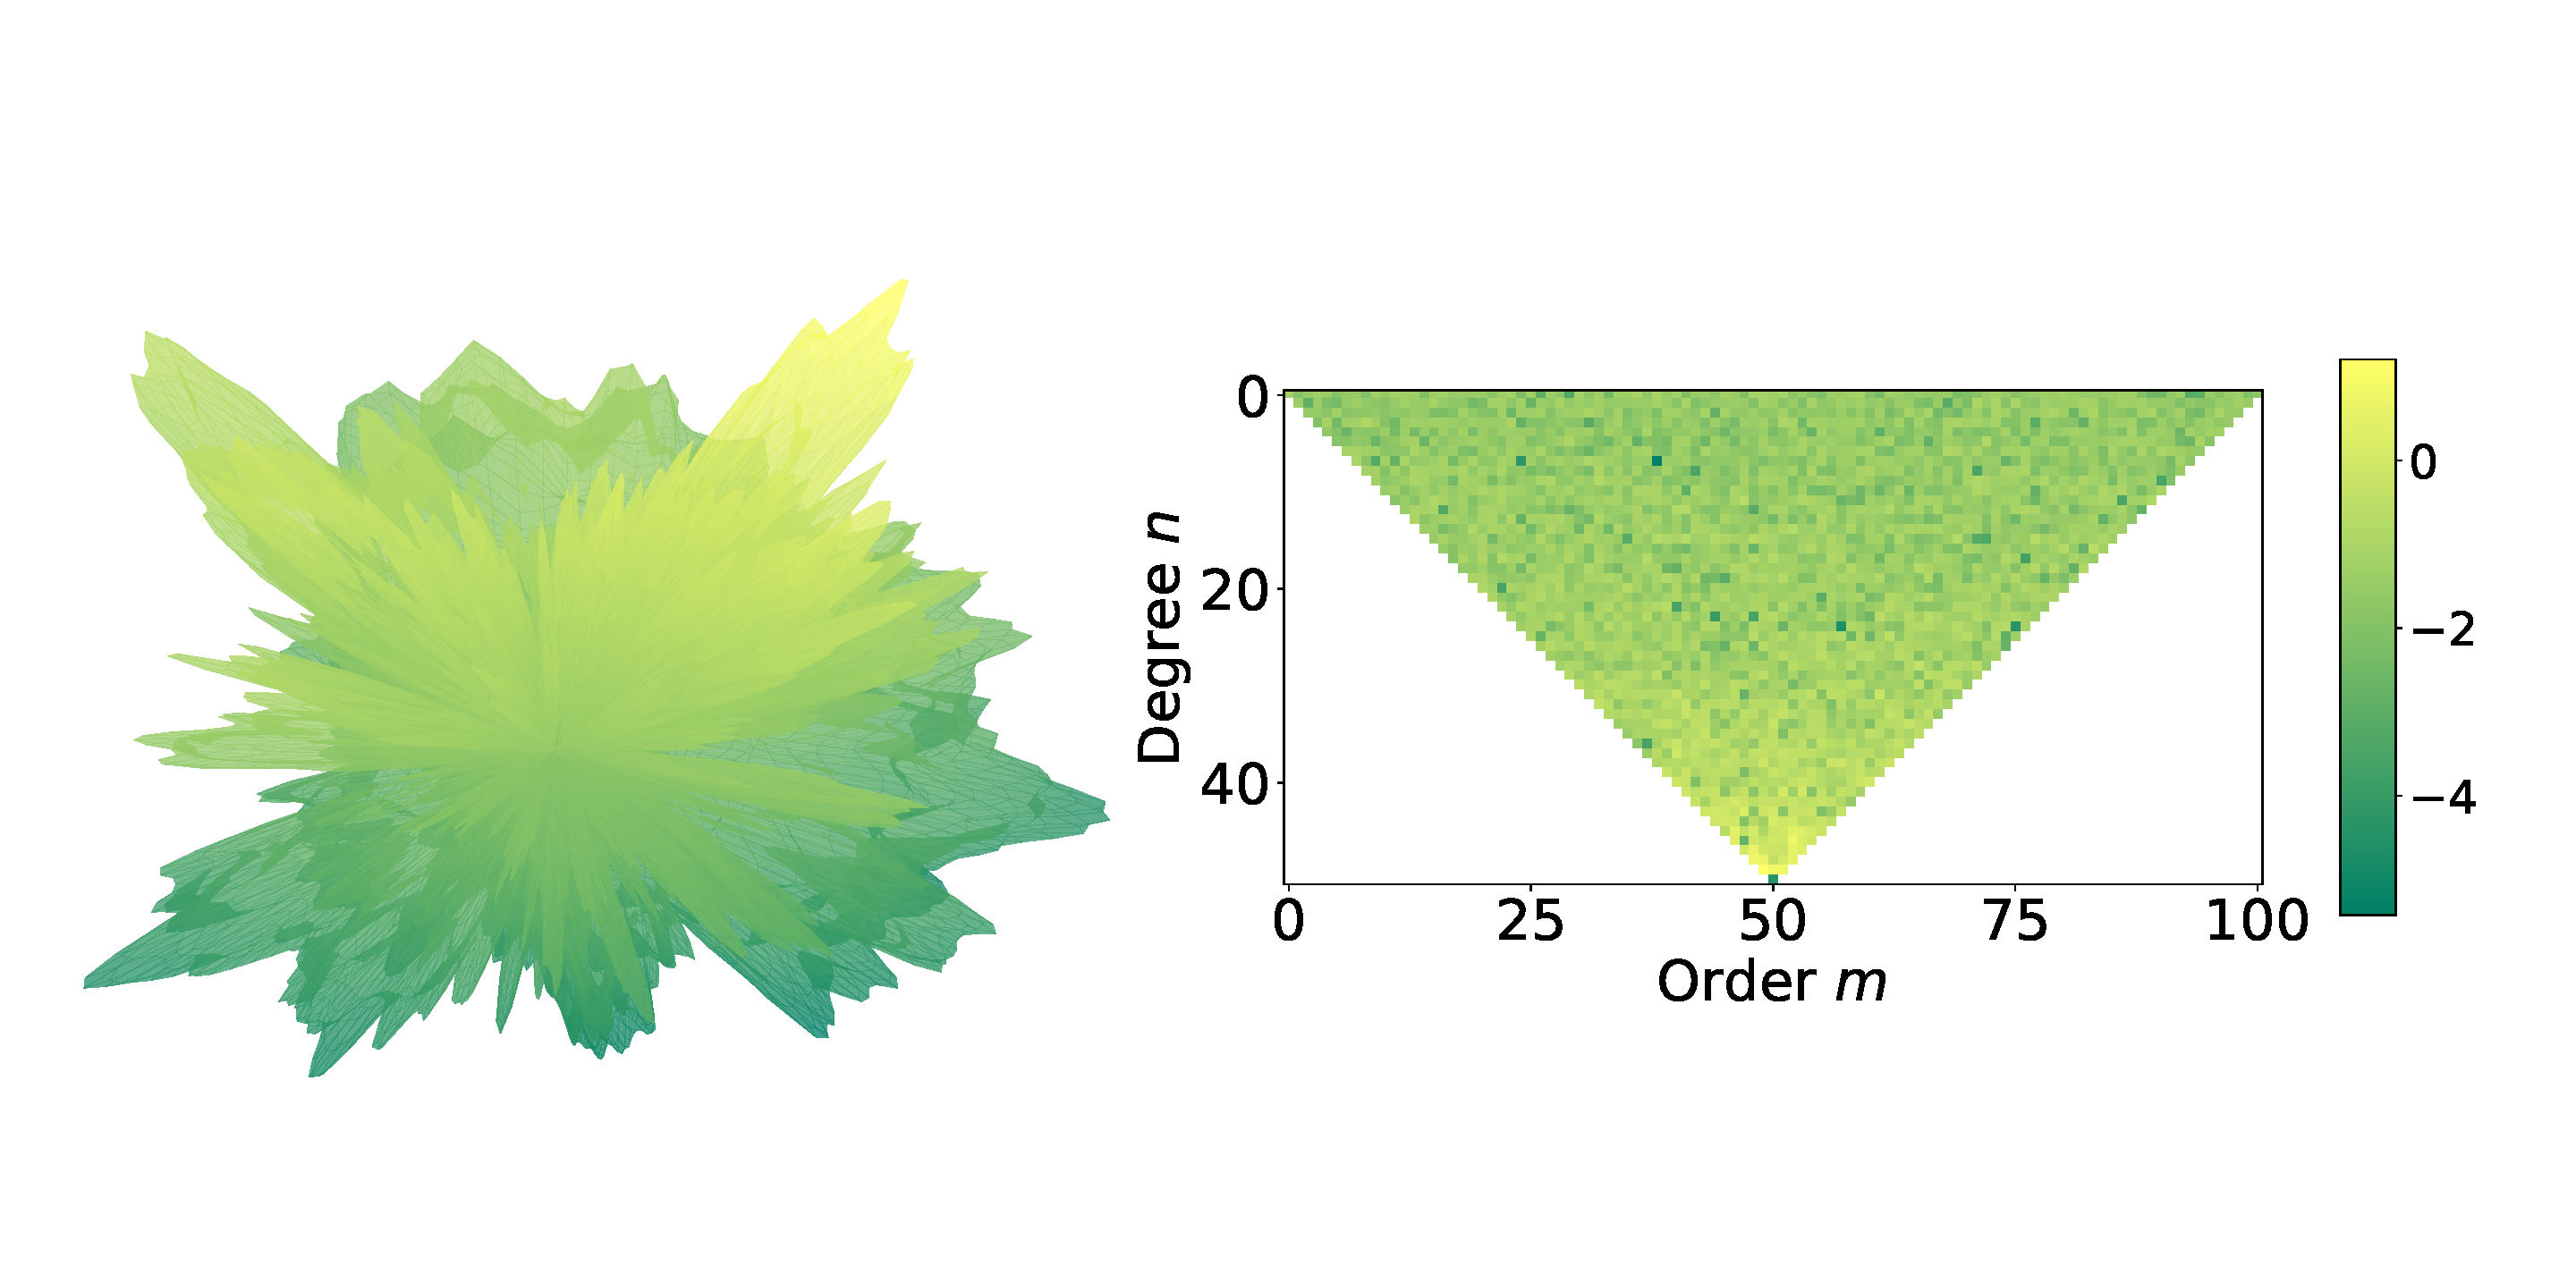
\includegraphics[width=.95\textwidth]{papers/kugel/figures/python/sph-fourier.pdf}
  \caption{
    A random spherical function is presented on the left plot, while the right
    plot shows its Fourier coefficients $c_{m,n}$. Notice the triangular
    structure of the right plot, which is a consequence of the constraint
    $|m|\leq n$.
    \label{kugel:fig:sph-fourier}
  }
\end{figure}

\begin{figure}
  \centering

  \noindent
  \subfigure[$N=0$]{\includegraphics[width=.25\linewidth, trim=700 0 700 100, clip]%
    {papers/kugel/figures/python/earth-fourier-decomposition/n=0}}
  \hspace{.07\linewidth}
  \subfigure[$N=10$]{\includegraphics[width=.25\linewidth, trim=700 0 700 100, clip]%
    {papers/kugel/figures/python/earth-fourier-decomposition/n=10}}
  \hspace{.07\linewidth}
  \subfigure[$N=50$]{\includegraphics[width=.25\linewidth, trim=700 0 700 100, clip]%
    {papers/kugel/figures/python/earth-fourier-decomposition/n=50}}

  \noindent
  \subfigure[$N=100$]{\includegraphics[width=.25\linewidth, trim=700 0 700 100, clip]%
    {papers/kugel/figures/python/earth-fourier-decomposition/n=100}}
  \hspace{.07\linewidth}
  \subfigure[$N=500$]{\includegraphics[width=.25\linewidth, trim=700 0 700 100, clip]%
    {papers/kugel/figures/python/earth-fourier-decomposition/n=500}}
  \hspace{.07\linewidth}
  \subfigure[$N=1000$]{\includegraphics[width=.25\linewidth, trim=700 0 700 100, clip]%
    {papers/kugel/figures/python/earth-fourier-decomposition/n=1000}}

  \caption{
    Reconstruction of a function on the surface of the sphere using a finite
    number of coefficients ($N$); with a higher number of coefficients more high
    frequency details appear. The function is the gravitational field of the
    earth measured by the GOCE mission.
    \label{kugel:fig:fourier-on-sphere-increasing-index}
  }
\end{figure}

The same logic can be extended to the spherical harmonic coefficients $c_{m,n}$.
In figure \ref{kugel:fig:fourier-on-sphere-increasing-index} we can see the same
concept as in figure \ref{kugel:fig:1d-fourier} but with a function
$f(\vartheta, \varphi)$ on the sphere. In this case we define the ``spectrum''
of the spherical function $f(\vartheta, \varphi)$ as the relation between
$c_{m,n}$ and the two indices $m$ and $n$. We can observe the same behaviour as
in the one dimensional Fourier case: the absolute value $|c_{m,n}|$ decays quite
quickly as $n$ increases. Thus, the coefficients with a higher $n$ index are
responsible for the small high-frequency details of the considered function.

This trend suggests a possible application: one could use these coefficients as
a compression technique. If extremely high resolution is not required, only the
lower ``frequency'' coefficients could be used to save memory, as is done in
digital lighting techniques \cite{SH_lighting_paper}.

\subsection{Energy of a Function $f(\vartheta, \varphi)$}

The decomposition of functions using spherical harmonics is not the only thing
we can extract from the orthogonality properties of the functions $Y^m_n$. The
aim of this section is to present another property you probably already know
from the classical Fourier theory in one dimension. It has to do with what is
usually referred to as the ``power'' of a signal (function) and it can be
expressed with the following theorem, that takes the name of \emph{Parseval's
theorem}.

\begin{theorem}[Parseval's theorem]
  \label{kugel:thm:parseval-1D}
  Suppose $f \in L^2$ is a complex valued $T$-periodic function, that has a
  Fourier series with coefficients $c_n$, then
  \begin{equation}
    \frac{1}{T}\int_T |f(x)|^2dx
    = \sum_{n \in \mathbb{Z}} |c_n|^2. 
    \label{kugel:eqn:parseval-1D}
  \end{equation}
\end{theorem}
\begin{proof}
  The proof is analogous to the two dimensional case (below) and is therefore omitted.
\end{proof}

In physics this is just another way to show that power\footnote{In physics and
engineering, the power of a signal (function) is usually defined to be the
derivative of the energy of a function, which is $\int | f(x) |^2 \, dx$.
However, if the function is periodic with period $T$, the power is defined to be
$\frac{1}{T} \int_T |f(x)|^2 \, dx$.} is conserved, so we could call it
``conservation theorem''. We know that the Fourier series is a way to map a
function in time domain to one in frequency domain, and most importantly, this
mapping is reversible (or invertible). The function we are considering still the
same but in the time domain is continuous and, in the case of the Fourier
series, in the frequency domain a discrete one.

We may have overused the term ``beautiful'', but we are not afraid to use it yet
again, because in our humble opinion this theorem is one of the more
understandable links between continuous and discrete. The conservation of power
in this case doesn't care about continuity or discreteness. The latter goes
through these two worlds, since on the left side of
\eqref{kugel:eqn:parseval-1D} we have an integral and on the right one we have a
summation. So, we can unify these two concepts with an equality and two
different representations of the same thing, namely the power of $f(x)$.  Now,
as you can imagine, it is possible to write an analog to theorem
\ref{kugel:thm:parseval-1D} on the surface of the sphere.

\begin{theorem}[Parseval's theorem on $\partial S$]
  \label{kugel:thm:parseval-sph}
  Suppose $f: S^2 \to \mathbb{C}$, that $f \in L^2$, and that $f$ has a Fourier
  series expansion with coefficients $c_{m,n}$, then
  \begin{equation}
    \label{kugel:eqn:parseval-sph}
    \int_0^{2\pi}\int_0^\pi |f(\vartheta, \varphi)|^2
      \sin\vartheta \, d\varphi \, d\varphi
    = \sum_{n=0}^\infty \sum_{m=-n}^n |c_{m,n}|^2.
  \end{equation}
\end{theorem}
\begin{proof}
  This is a special case of theorem \ref{kugel:thm:general-parseval-sph} (below).
\end{proof}

To prove what we just stated, we want to consider a more general case, namely
theorem \ref{kugel:thm:general-parseval-sph}.  Having proved the latter, it will
follow that Parseval's theorem \ref{kugel:thm:parseval-sph} is also correct.

\begin{theorem} %[General Parseval's theorem on $\partial S$]
  \label{kugel:thm:general-parseval-sph}
  Suppose $f(\vartheta, \varphi)$ and $g(\vartheta, \varphi)$ are both complex
  valued functions in $L^2$, that have a Fourier series expansion with the
  coefficients $c_{m,n}$ and $c_{m',n'}$ respectively, then
  \begin{equation}
    \label{kugel:eqn:general-parseval-sph}
    \left\langle f, g\right\rangle_{\partial S}
    = \int_0^{2\pi}\int_0^\pi
      f(\vartheta, \varphi) \overline{g(\vartheta, \varphi)}
      \sin\vartheta \, d\varphi \, d\varphi 
    = \sum_{n=0}^\infty\sum_{m=-n}^n c_{m,n}\overline{c_{m',n'}}.
  \end{equation}
\end{theorem}
\begin{proof}
  We can assume that both functions $f(\vartheta, \varphi)$ and $g(\vartheta,
  \varphi)$ have a spherical harmonics series expansion, hence:
  \begin{align*}
    f(\vartheta, \varphi) &= \sum_{n=0 }^\infty \sum_{m =-n }^{n }
      c_{m, n } Y^{m }_{n }(\vartheta, \varphi), &
    g(\vartheta, \varphi) &= \sum_{n'=0}^\infty \sum_{m'=-n'}^{n'}
      c_{m',n'} Y^{m'}_{n'}(\vartheta, \varphi).
  \end{align*}
  By computing their inner product we obtain
  \begin{align*}
    \left\langle f, g\right\rangle_{\partial S}
    = \int_0^{2\pi}\int_0^\pi
      f(\vartheta, \varphi)\overline{g(\vartheta, \varphi)}
      \sin\vartheta \, d\varphi \, d\varphi 
    &= \left\langle
        \sum^\infty_{m=0}\sum_{n=-m}^m c_{m,n} Y^m_n,
        \sum^\infty_{m'=0}\sum_{n'=-m'}^{m'} c_{m',n'} Y^{m'}_{n'}
      \right\rangle_{\partial S} \\
    &= \sum_{m=0}^\infty \sum_{n=-m}^m \sum_{m'=0}^\infty \sum_{n'=-m'}^{m'} c_{m',n'}\overline{c_{m,n}} \left\langle Y^m_n,  Y^{m'}_{n'} \right\rangle_{\partial S}.
  \end{align*}
  Since the spherical harmonics are orthonormal, only the terms of the sum in
  which $m=m'$ and $n=n'$ survive, leading to
  \begin{equation*}
    \int_0^{2\pi}\int_0^\pi
      f(\vartheta, \varphi)\overline{g(\vartheta, \varphi)}
      \sin\vartheta \, d\varphi \, d\varphi 
    = \sum_{n=0}^\infty\sum_{m=-n}^n
      c_{m,n}\overline{c_{m',n'}}. \qedhere
  \end{equation*}
\end{proof}

With this last theorem, we have given more generality to the Parseval's theorem.
In this way, we are not only able to calculate the power of a function using its
spherical harmonic coefficients, but also the possibility to compute other
things such as the cross correlations of two functions using, simply the sum of
the multiplications of their spherical harmonic coefficients.
